\documentclass[12pt]{article}
\usepackage[english]{babel}
\usepackage{graphicx}
\usepackage{framed}
\usepackage[normalem]{ulem}
\usepackage{amsmath}
\usepackage{amsthm}
\usepackage{amssymb}
\usepackage{amsfonts}
\usepackage{enumerate}
\usepackage{graphicx} % Allows including image
\usepackage{hyperref}
\hypersetup{
  linkcolor  = blue,
  citecolor  = blue,
  urlcolor   = blue,
  colorlinks = true,
} % color setup
\usepackage[utf8]{inputenc}
\usepackage[margin=1in]{geometry}
\usepackage{float} % for "H" placement specifier
\usepackage[authoryear]{natbib}
\usepackage{indentfirst}
\usepackage[dvipsnames]{xcolor}
\usepackage{float}
\usepackage{array}


\usepackage[T1]{fontenc}
\usepackage{tikz}
\newcommand{\fatterdot}{\raisebox{0.15ex}{\tikz\filldraw[black,x=1.5pt,y=1.5pt] (0,0) circle (1);}}

\DeclareUnicodeCharacter{FB01}{fi}
\DeclareUnicodeCharacter{FF0C}{,}
\DeclareMathOperator*{\Prob}{P}
\DeclareMathOperator*{\argmax}{arg\,max}
\DeclareMathOperator*{\argmin}{arg\,min}
\setlength\extrarowheight{1pt}

\newcommand\red[1]{{\color{red}#1}}

\bibliographystyle{plainnat}

\newtheorem{theorem}{Theorem}[section]
\newtheorem{corollary}{Corollary}[theorem]
\newtheorem{lemma}[theorem]{Lemma}
\newtheorem{prop}[theorem]{Proposition}
\newtheorem{defn}[theorem]{Definition}
\allowdisplaybreaks

\title{Condition for Theorem 3.2}

\date{}

\begin{document}

\maketitle

When $\frac{n_1}{N_1} \geq \frac{n_2}{N_2}$ and $k = j$, then 

$$g_{n_1, k} \circ g_{n_2, j}^{-1}(t) - g_{N_1, k} \circ g_{N_2, j}^{-1}(t)$$ is non-negative when $t \in (0,1),$ where $g_{n,i}(x) = I_x(i, n-i+1)$, $I_x(\alpha, \beta)$ is the CDF of Beta$(\alpha, \beta)$ distribution. 

We hope to find a sufficient condition of $g_{n_1, k} \circ g_{n_2, j}^{-1}(t) - g_{N_1, k} \circ g_{N_2, j}^{-1}(t)$ is non-negative when $t \in (0,1)$. 

Define the function $f(x) = g_{n_1, k}(x) - g_{N_1, k}(x), x \in (0,1), n_1 \geq N_1$ and we will prove $f(x) \geq 0$ for all $x \in (0,1)$

\begin{proof}
	we find $f(0) = 0$ and $f(0) = 0$, then it suffices to show $f^`(x)$ is positive first and then becomes negative. 
	
	\begin{align*}
		f^`(x) &= \frac{x^{k-1}(1-x)^{n_1 - k}}{B(k, n_1+1-k)} - \frac{x^{k-1}(1-x)^{N_1 - k}}{B(k, N_1+1-k)} \\
		&=  \frac{x^{k-1}(1-x)^{N_1 - k}}{B(k, n_1+1-k)}((1-x)^{n_1 - N_1} - \frac{B(k, n_1+1-k)}{B(k, N_1+1-k)})
	\end{align*}

When $x = 0$, $(1-x)^{n_1 - N_1} = 1$ and when $x = 1$, $(1-x)^{n_1 - N_1} = 0$. Also $\frac{B(k, n_1+1-k)}{B(k, N_1+1-k)} \leq 1$. 

Then $f^`(x)$ is positive first and then becomes negative. And now we have $f(x) \geq 0$ for all $x \in (0,1)$.

Then when $x = g_{n_2, j}^{-1}(t)$, where $t \in (0,1)$, we have
\begin{equation} \label{eq:inequa1}
	g_{n_1, k}(g_{n_2, j}^{-1}(t)) \geq g_{N_1, k}(g_{n_2, j}^{-1}(t))
\end{equation}
Since $g_{N_1, k}(x)$ is an increasing function and $g_{n_2, j}^{-1}(t) \geq g_{N_2, j}^{-1}(t)$ when $n_2 \leq N_2$

Now we have 

\begin{equation} \label{eq:inequa2}
	g_{N_1, k}(g_{n_2, j}^{-1}(t)) \geq g_{N_1, k}(g_{N_2, j}^{-1}(t))
\end{equation}

Based on \ref{eq:inequa1} and \ref{eq:inequa2}, we have 

\begin{equation} \label{eq:inequa2}
	g_{n_1, k}(g_{n_2, j}^{-1}(t)) \geq g_{N_1, k}(g_{N_2, j}^{-1}(t))
\end{equation}

\begin{figure}
	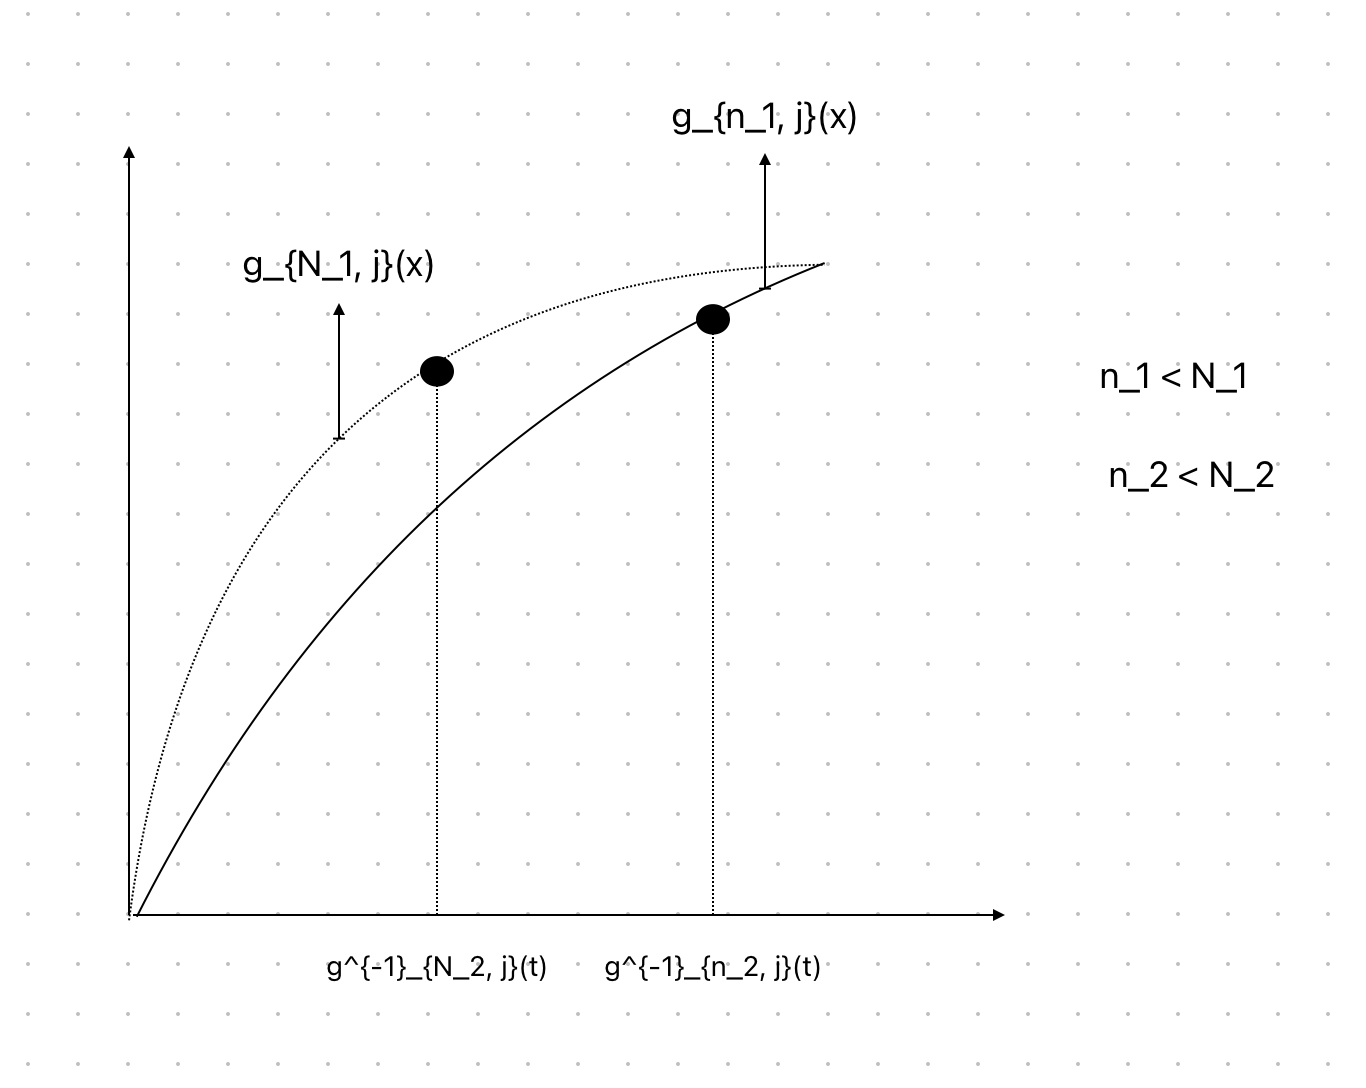
\includegraphics[scale = 0.7]{conditions.png}
\end{figure}

\end{proof}

































\end{document}